\documentclass[11pt]{amsart}
\usepackage[spanish]{babel}
\usepackage[latin1]{inputenc}
\usepackage[T1]{fontenc}
\usepackage{geometry}                % See geometry.pdf to learn the layout options. There are lots.
\geometry{letterpaper}                   % ... or a4paper or a5paper or ... 
%\geometry{landscape}                % Activate for for rotated page geometry
%\usepackage[parfill]{parskip}    % Activate to begin paragraphs with an empty line rather than an indent
\usepackage{graphicx}
\usepackage{amssymb}
\usepackage{epstopdf}
\usepackage{hyperref}
\usepackage{epigraph}
\usepackage[all]{hypcap}


\title{Segmentaci\'on de im\'agenes mediante un sistema din\'amico discreto.}
\author{Sergio Arbeo}
%\date{}                                           % Activate to display a given date or no date

\begin{document}
\maketitle
\section{Motivaci\'on}
Un sistema de OCR (Optical Character Recognition o reconocimiento \'optico de caracteres) consta de varias
partes desde que se introduce una texto-imagen hasta que devuelve el texto en s\'i.\\

Una primera etapa es un tratamiento previo de la imagen para despu\'es pasar a la segmentaci\'on de la imagen.
Dicha segmentaci\'on busca descomponer la imagen en diferentes partes. En el caso del OCR, despu\'es se buscar\'a
dar sentido a dichos segmentos.\\

\section{R\'apida introducci\'on a un tratamiento previo de la imagen.}

El principal problema con la segmentaci\'on de im\'agenes es que una letra no tiene porqu\'e componerse de un
\'unico trazo. El ejemplo m\'as sencillo de ver es la de la \emph{i latina}, la cual se compone de dos segmentos
diferenciados: el trazo principal y el punto.\\

Afortunadamente hay bastante literatura en c\'omo tratar con estos casos. De forma breve se expondr\'an las dos
herramientas b\'asicas para tratar con dicho problema. Se ha de notar que ambos procesos se realizan sobre
im\'agenes binarias, en las cuales interior y exterior se identifican con uno de los dos colores. Normalmente,
blanco se corresponde con el interior y el negro con el exterior.\\

\begin{itemize}
\item Erosi\'on: Dicho proceso reduce el tama\~no del interior del objeto pasando al exterior los p\'ixeles m\'as cercanos al borde.\\
\item Dilataci\'on: Este proceso es el contrario a la erosi\'on. En este caso, los p\'{i}xeles m\'as cercanos
del exterior se a\~naden al interior.
\end{itemize}

Adem\'as, encontramos dos combinaciones importantes de estos dos procesos:\\

\begin{itemize}
\item Apertura: Se realiza una erosi\'on seguida de una dilataci\'on. Este proceso elimina los objetos m\'as
peque\~nos manteniendo la forma de los grandes.
\item Clausura: Se realiza una dilataci\'on seguida de una erosi\'on. Este proceso une segmentos separados pero
cercanos, a la vez que elimina posible ruido.
\end{itemize}

A la hora de realizar un OCR la interesante es la clausura. Tambi\'en se ha de observar que los procesos de
erosi\'on y dilataci\'on pueden realizarse en distintas direcciones.\\

\section{Primera aproximaci\'on al sistema neuronal.}

\subsection{Introducci\'on.}

El presente trabajo se basa en el paper \emph{Discrete-Time Dynamic Image-Segmentation System} escrito por Ken'ichi
Fujimoto, Mio Kobayashi, y Tetsuya Yoshinaga de la Universidad de Tokushima en Jap\'on. En dicho paper se propone
modelo de una neurona y una arquitectura de varias de esas neuronas. Adem\'as, proponen una arquitectura para
lo que se denomina segmentaci\'on din\'amica de im\'agenes. Esto no es m\'as que la fragmentaci\'on de una imagen
no est\'atica, sino a lo largo del tiempo.\\

\subsection{Sistema de una neurona.}

El sistema propuesto en el paper es el siguiente (la notaci\'on se ha cambiado para adaptarla a la utilizada
en clase).

$$
x_{t+1}=k_{f}x_{t}+d+W_{x}\cdot g(x_{t}+y_{t},\theta_{c})-W_{z}\cdot g(z_{t},\theta_{z})
$$

$$
y_{t+1}=k_{r}y_{t}-\alpha\cdot g(x_{t}+y_{t},\theta_{c}) + a
$$

$$
z_{t+1}=\phi\left\{g\left( g(x_{t}+y_{t},\theta_{f}),\theta_{d}\right) -z_{t} \right\}
$$

Se da que $t\in\mathbb{Z}$ es el tiempo discreto y que $g(\cdot , \cdot)$ es la funci\'on salida de neurona,
la cual se puede expresar f\'acilmente a partir de la sigmoidal.\\

$$
g(u_{t},\theta)=P(\frac{-(u_{t}-\theta)}{\epsilon})
$$

Siendo $\epsilon$ el gradiente de $g$ en $u_{t}=\theta$.\\\\

Antes de pasar a de pasar a describir los par\'ametros, se ha de observar que el modelo se basa en dos variables
de estado ($x$ e $y$) y un inhibidor ($z$). Esto facilita la explicaci\'on de los distintos par\'ametros.\\

Los coeficientes $k_{f}$, $k_{r}$ y $\phi$ se corresponden respectivamente con los gradientes de $x$, $y$ y $z$.
$W_{x}$ y $\alpha$ son \emph{self-feedback gains}? de las variables internas. La $W_{z}$ indica el nivel de
acoplamiento entre las variables internas y el inhibidor. Las distintas $\theta$ son umbrales; en el caso de
$\theta_{c}$ se corresponde al umbral de la funci\'on de salida $g$ de la neurona y $\theta_{z}$ al de la salida
del inhibidor. M\'as sutil es la diferencia entre $\theta_{f}$ y $\theta_{d}$: el primero es el umbral en el
que se considera que una neurona ha sido disparada mientras que el segundo es el que detecta dicho disparo en
el inhibidor, de ahí que haya una funci\'on de salida anidada en la ecuaci\'on de $z_{t+1}$.\\\\

En el paper se puede encontrar un ejemplo de ejecuci\'on para ver los efectos del inhibidor. Los par\'ametros
as\'i como los valores iniciales se pueden consultar en el propio paper. En la figura~\ref{fig:oscillator-effect}
se puede observar c\'omo cuando la neurona supera el umbral (en este caso $\theta_{f}=15$) el inhibidor entra
en acci\'on disminuyendo el m\'odulo del valor (en este caso, la suma de las variables internas).

\begin{figure}[h]
\centering
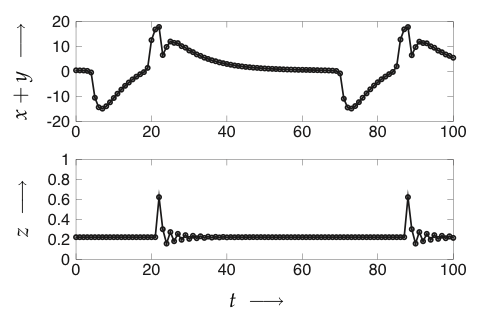
\includegraphics[width=0.5\textwidth]{img/oscillator-effect.png}
\caption{Efectos del inhibidor.}
\label{fig:oscillator-effect}
\end{figure}

\section{Siguientes pasos.}

Tras una primera lectura del art\'{i}culo, me encuentro estudiando el apartado 2.2 en el cual se plantea una
arquitectura de neuronas y se modifica el sistema puesto que las neuronas est\'as dispuestas en forma de rejilla
y conectadas con sus cuatro vecinas. Es una parte que no termino de comprender c\'omo funciona.\\

Despu\'es, probablemente corresponda una implementaci\'on b\'asica en el ordenador de forma que se puedan hacer
simulaciones y tener una parte pr\'actica del an\'alisis del sistema destinado a la elecci\'on de los par\'ametros,
que es la siguiente parte del trabajo.\\

Finalmente, se pasar\'an a estudiar las aplicaciones pr\'acticas del mismo.

\section{Conclusiones.}

De la primera lectura en general y del estudio parcial empiezo a vislumbrar que este sistema no es una buena
aproximaci\'on para el problema de segmentaci\'on aplicado al problema del OCR, pues para encontrar un n\'umero
indeterminado de fragmentos se requiere aplicar varias veces el sistema e ir fragmentando la imagen en partes
cada vez m\'as peque\~nas.
\end{document}
